\chapter{Metodologia} 
\label{cap:metodologia}

%O objetivo deste trabalho é desenvolver um sistema de navegação autônoma baseado em
%visão computacional a fim de capacitar um veículo terrestre a se locomover em ambientes externos
%não estruturados, ou seja, um campo com vegetação/plantação e/ou floresta pouco densa. O veículo
%deverá ser capaz de desviar de obstáculos de forma autônoma, e se dirigir até uma
%localização determinada escolhendo por meios próprios o caminho a seguir. Deverá ter alguma
%capacidade de reconhecer o terreno que irá se deslocar a fim de evitar zonas não transponíveis ou
%muito acidentadas.

No capítulo anterior foram apresentados os principais problemas referentes a
navegação autônoma do veículo relativos às questões de localização, mapeamento e
navegação. Em relação a localização, está sendo considerada uma proposta de
utilização de sensores do tipo GPS e bússola e de uma câmera estéreo para o
mapeamento e desvio de obstáculos. Baseado nas referências analisadas, os
métodos VFH e RNAs são soluções adequadas para uma navegação baseada em uma
orientação de destino, associada ao desvio de obstáculos detectados através de
uma percepção local. Em \cite{caio} foi utilizado o VFH para desvio de
obstáculos utilizando como informação sensorial dados de uma câmera estéreo. O
histograma polar utilizado pelo método VFH foi gerado a partir da informação de
profundidade obtida pela câmera estéreo. 


%Estes elementos constituem-se portando
%dos módulos e componentes deste projeto, onde as ferramentas usadas e a
%arquitetura geral do sistema serão detalhadas a seguir.

%de pesquisa de mestrado. No capítulo seguinte será apresentada a metodologia proposta.


No sistema RoBombeiros \cite{Pessin2008} foi implementada uma solução baseada em
coordenadas GPS para localização e uma RNA para o controle e navegação. O
sistema foi projetado para ambientes externos onde os veículos tinham como meta
o combate à incêndios florestais. Este sistema foi testado apenas em simulação
que consistia em ambientes não estruturados onde a vegetação predominante
era composta por árvores. Os veículos foram capazes de desviar dos obstáculos
adequadamente e se dirigir ao destino estabelecido (\fig{fig:incendio}). 


\begin{figure}[ht]
	\begin{minipage}[b]{0.95\linewidth}
	    \centering
	    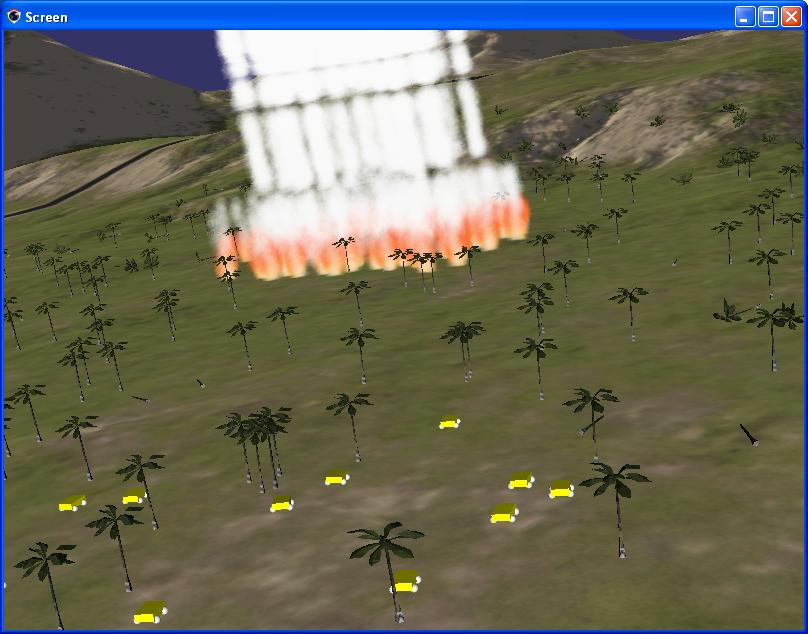
\includegraphics[width=12cm]{images/fogo30905osg.jpg}
	 	\caption{RoBombeiros - Navegação em ambiente não estruturado e estratégia de
	 	combate a incêndio florestal.}
	 	\label{fig:incendio}
	\end{minipage}
\end{figure}

Apesar do trabalho de \cite{Pessin2008} ter dado grande foco no combate à
incêndios e nas estratégias de deslocamento e atuação de um grupo de veículos,
este projeto irá se focar em um único veículo. Para os testes práticos será
avaliada apenas a capacidade de chegada ao destino com sucesso, dado que para
os experimentos em ambiente real somente a navegação estará sendo validada.


%Estes elementos constituem-se portando dos módulos e componentes deste projeto,
%onde as ferramentas usadas e a arquitetura geral do sistema serão detalhadas a
%seguir.

%\section{Objetivos Específicos}

Os principais objetivos específicos deste projeto de mestrado, que se apresentam
como um desdobramento do objetivo geral descrito acima, são:

\begin{itemize}

\item Extração de referenciais a partir de um par de câmeras, constituindo um
sistema de visão binocular (estéreo);

\item Propor melhorias nos algoritmos de geração do mapa de disparidade, obtido
a partir das imagens estéreo;

\item Gerar um mapa de navegabilidade local a partir de informações visuais;
%,
%que possa ser adaptado a algoritmos de planejamento e controle de navegação
%autônoma;

\item Desenvolver um mecanismo de navegação autônoma, baseado nas informações de
GPS, Bússola e do Sistema de Visão, capaz de desviar de obstáculos e dirigir o
veículo até um destino determinado de forma robusta e eficiente;

\item Fazer uso dos conhecimentos prévios de trabalhos desenvolvidos no
laboratório e contribuir para a consolidação de tecnologias capazes de atribuir
navegabilidade autônoma a veículos de diversas naturezas para fins práticos;

\item Aplicação e avaliação do sistema de navegação autônoma em um veículo real
em ambiente externo não estruturado.

\end{itemize}

%2012-10-15 Revisar
%\section{Discussão}

\section{Materiais e Métodos}

Este trabalho será desenvolvido junto ao LRM\foot{LRM - Laboratório de Robótica
Móvel do ICMC/USP - http://www.lrm.icmc.usp.br} – Laboratório de Robótica Móvel
do ICMC/USP. Diversos trabalhos relacionados ao desenvolvimento de veículos
autônomos e robôs móveis inteligentes vêm sendo pesquisados e desenvolvidos
junto a este laboratório, destacando-se, a pesquisa e uso de sistemas de
navegação baseados em visão computacional.
% Atualmente, o Laboratório conta com uma parceria estabelecida com a empresa
% Jacto S/A\foot{Grupo Jacto - http://www.jacto.com.br} (equipamentos agrícolas)
% para o desenvolvimento de um sistema autônomo de navegação de veículos em
% ambientes agrícolas.
O LRM possui atualmente duas plataformas de teste para aplicações de veículos
móveis autônomos que foram adquiridas pelo INCT-SEC: os veículos CaRINA I e
CaRINA II\foot{CaRINA - Carro Robótico Inteligente para Navegação Autônoma -
http://www.lrm.icmc.usp.br}
% (fig. 3.1).
% Também, possui robôs e plataformas móveis de pequeno porte.
Para realizar as atividades de validação em ambiente real será utilizada a
plataforma CaRINA I (\fig{fig:carina}) que possui a automatização dos seus controles de frenagem,
aceleração e esterçamento. O veículo CaRINA I é o mais adaptado para ambientes
externos não estruturados (\textit{off-road}), já o veículo CaRINA II é mais
focado para ambientes urbanos (vias e estradas urbanas).

\vspace{0.5cm}
\begin{figure}[!h]
  	\centering
	%\begin{minipage}[b]{0.33\linewidth}
	    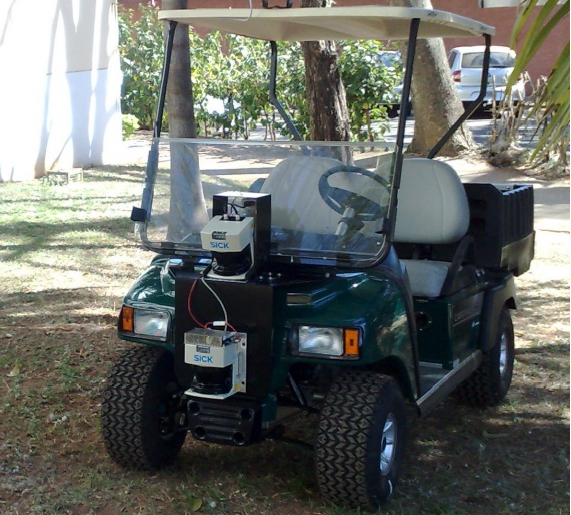
\includegraphics[width=8cm,height=7cm]{images/carina_1.png}
	 	\caption{CaRINA I - Carro elétrico automatizado.}
		\fonte{LRM (divulgação)}
	 	\label{fig:carina}
 	%\end{minipage}
\end{figure}

%Para realizar os
%testes e avaliar o desempenho do sistema proposto teremos à disposição o veículo
%CaRINA I, que já possui integrada uma câmera de vídeo estéreo e um dispositivo
%de localização GPS com bússola, bem como outros dispositivos sensores e
%atuadores de controle do veículo. O veículo CaRINA I é o mais adaptado para
%ambientes externos não estruturados (off-road) a que pretendemos aplicar. Já o
%veículo CaRINA II está mais focado para ambientes urbanos (vias e estradas
%urbanas).

A primeira etapa do projeto consiste no levantamento de todos os pontos críticos
do sistema proposto, após esta etapa serão avaliadas as técnicas mais acessíveis
que são adequadas para o tratamento de cada ponto crítico. Será levado em conta
prioritariamente o que já vem sendo trabalhado no laboratório, a fim de promover
a integração das tecnologias já dominadas pelo grupo.
% Para a programação serão utilizadas as bibliotecas OpenCV\foot{OpenCV -
% http://opencv.willowgarage.com/} e PCL\foot{PCL - http://pointclouds.org} como
% ferramentas centrais.
% , podendo vir a ser utilizado o framework ROS\foot{ROS - http://www.ros.org}
% para a integração destas ferramentas.
Para a localização global será aplicada basicamente a utilização de GPS e
bússola. Como o destino também será dado em forma de informação de posição de
GPS esta questão não é tão crítica para esse projeto. A localização é bastante
afetada por ruídos dos sensores, principalmente aqueles que fornecem informações
de odometria. Dependendo da aplicação pode ser desnecessário considerar uma
localização espacial precisa do veículo, apenas que o mesmo seja capaz de chegar
no seu destino eficazmente. Por se tratar de um ambiente externo e não
estruturado, sua navegação permite uma certa liberdade de movimentos dentro de
um perímetro onde haja um caminho factível, preferencialmente buscando um
caminho próximo do ótimo, como é o caso deste trabalho. Desta forma, o erro
associado ao posicionamento por GPS não está sendo considerado crítico.

%Em relação ao sistema de controle do veículo está sendo considerada uma 
%abordagem primeiramente deliberativa, onde as trajetórias serão planejadas de acordo com 

A abordagem da visão computacional se insere como principal fonte de informação
sensorial do ambiente no contexto deste projeto. Inicialmente serão estudados e
trabalhados algoritmos para a criação do mapa de disparidade a partir do par de
imagens obtidas da câmera estéreo.
% Neste processo, o algoritmo deverá ter um compromisso de desempenho entre a
% qualidade do mapa de disparidade/profundidade e a performance em termos de
% tempo de processamento.
A partir do mapa de disparidade será elaborado um mapa de navegabilidade, que
representa as regiões navegáveis (seguras) e regiões não navegáveis (obstáculos
e regiões a evitar) em frente ao veículo. O mapa final gerado será utilizado em
conjunto com as informações de posição atual e de destino (GPS e bússola), a fim
de realizar a navegação do veículo.


A primeira abordagem na construção de mapas de navegabilidade a partir de
informações visuais será pesquisada a viabilidade de se gerar mapas de
profundidade menos densos a cada instante de tempo com o propósito de reduzir o
custo computacional desta técnica. Para tal pretende-se utilizar a estratégia de
foco de atenção, onde apenas uma região de maior interesse é analisada a cada
momento. Como o veículo está em movimento o foco de atenção é constantemente
atualizado, com isso espera-se obter um mapeamento do ambiente de forma
incremental suficiente para o planejamento da navegação.

Serão desenvolvidos estudos relacionados à aplicação de técnicas de campos
potenciais e de algoritmos derivados do VFH, a fim de realizar o planejamento e
controle da navegação do veículo autônomo. Além destes estudos, também serão
desenvolvidos estudos relativos ao uso de Redes Neurais Artificiais (RNAs) para
o controle da navegação do veículo, conforme proposto no trabalho dos
RoBombeiros. Ambas as técnicas, VFH e RNAs, são adequadas para uma navegação
baseada em um ponto/orientação de destino (fornecido pelas coordenadas GPS).
Assim, será possível inclusive comparar o desempenho e resultados obtidos com
cada uma destas técnicas, permitindo uma melhor avaliação e escolha do melhor
método a ser adotado no veículo autônomo.
Nestas duas abordagens serão consideradas como parâmetro de entrada as
informações tridimensionais do mapa de navegabilidade. Além disto, também serão
necessários estudos que visam identificar, a partir das imagens da câmera
estéreo, o plano de referência de base (chão), seus desníveis e impedimentos,
classificando-os como elementos transponíveis ou não. 

%Elemento que também é
%parâmetro para o planejamento, controle e estratégia da navegação.

%Para o desenvolvimento do sistema de navegação autônoma do veículo será
%utilizada a ferramenta Player-Stage\foot{Player Project e Player-Stage -
%http://www.willowgarage.com/pages/software/player e
%http://playerstage.sourceforge.net}, que já vem sendo adotada junto ao LRM (Wolf
%et al., 2009).
%Esta ferramenta permite desenvolver simulações dos robôs e veículos móveis
%baseadas no uso de sensores e atuadores virtuais equivalentes aos disponíveis no
%veículo. O software Player também provê ferramentas para o acesso aos
%dispositivos de hardware do robô, oferecendo uma interface (API) de alto nível
%para acesso aos drivers de dispositivos, como o GPS, a bússola, e os
%controladores dos motores do veículo. Esta ferramenta tem permitido um maior
%reaproveitamento de código e maior produtividade no desenvolvimento de
%aplicações robóticas junto ao LRM.

\textbf{O método de trabalho proposto neste trabalho consiste na execução
continuada das seguintes etapas:}

\begin{itemize}
\item Coleta de dados (ambiente real)
\item Simulação e análise com os dados coletados
\item Verificação (comportamento) em ambiente simulado 
\item Validação (ambiente real)
\end{itemize}


\subsection{Simulação}

Para este trabalho a simulação desempenhará papel essencial nos testes e na
avaliação das técnicas a serem utilizadas. Para tal será utilizada a plataforma
ROS\foot{ROS - Robotic Operating System - http://www.ros.org} que possui o
simulador físico 3D Gazebo. Esta plataforma está sendo considerara por estar
sendo adotada por diversos grupos de pesquisa na área da robótica. É uma
plataforma \textit{Open Source} que também tem servido de repositório para
compartilhar implementações de algoritmos propostos pela comunidade científica,
assim como \textit{drivers} de acesso aos dispositivos físicos, como sensores e
até mesmo plataformas robóticas completas (ex.
PR2\foot{PR2 - Personal Robot 2 - http://www.willowgarage.com}).

%OSORIO
%> Podia detalhar um pouco mais o ROS, descrevendo as facilidades que oferece,
% os recursos (log, drivers, simulação no gazebo, etc). Ficou muito resumido 
% e compacta esta parte. Não tem nem uma imagem do Carina I virtual !
% Imagino que esteja nos planos escrever mais sobre isto, mas desde já fica o
% pedido de mais detalhes aqui.

% A simulação neste contexto tem como principais vantagens e desvantagens:
\textbf{O uso da simulação no contexto deste projeto tem como principais aspectos:}

\begin{itemize}
\item Maior repetibilidade dos experimentos;
\item Replicação dos experimentos (e sem necessidade do equipamento físico);
\item Versatilidade (ex. troca de componentes, sensores, cenário, etc.).
\item Segurança (experimentos preliminares sem comprometer os equipamentos)
\end{itemize}

\textbf{Como desvantagens, a simulação pode ter os seguintes aspectos:}

\begin{itemize}
\item A modelagem dos cenários é custosa (tempo);
\item Não reflete fielmente a realidade.
\end{itemize}


A modelagem do sistema em um ambiente virtual é um passo fundamental para
executar experimentos em um simulador. Os experimentos em simulação podem ser
replicados e repetidos mais facilmente, desta forma, uma maior quantidade de
dados pode ser extraída para análises e verificação do comportamento dos
algoritmos. A maioria dos algoritmos utilizados no contexto da robótica móvel
autônoma requerem uma parametrização e um refino de diversos parâmetros para se
adequarem às necessidades da aplicação. Este refino está diretamente associado
aos comportamentos desejados que devem ser testados. Com o uso de simulação
estes parâmetros e seus efeitos podem ser melhor observados antes de se levar o
experimento para o ambiente real.

Para a plataforma CaRINA I que será utilizada já foram descritos os modelos de
simulação, do veículo e de alguns cenários de testes (\fig{fig:model},
\fig{fig:gazebo}).

\begin{figure}[ht]
	\begin{minipage}[b]{0.4\linewidth}
	    \centering
	    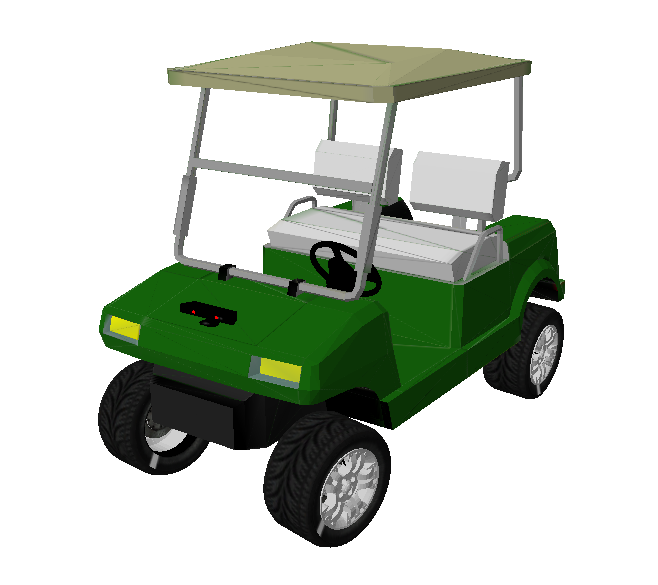
\includegraphics[width=8cm]{modelo_carina/carina_rviz_fundo_branco_sem_grid.png}
	 	\caption{CaRINA I - modelo virtual}
	 	\label{fig:model}
	\end{minipage}
	\hspace{1cm}
	\begin{minipage}[b]{0.4\linewidth}
	    \centering
	    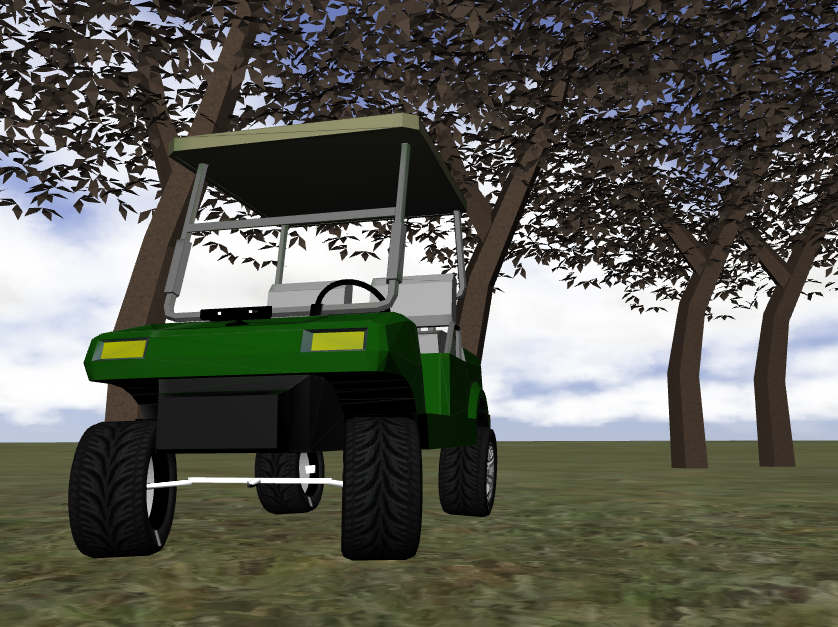
\includegraphics[width=8cm]{modelo_carina/carina_gazebo_frente_fundo.png}
	 	\caption{CaRINA I - cenário de ambiente não estruturado}
	 	\label{fig:gazebo}
	\end{minipage}
\end{figure}

Para a modelagem de robôs na plataforma ROS é utilizada uma linguagem para a
descrição chamada URDF (\textit{Unified Robot Description Format}). O URDF é
uma linguagem de descrição em XML onde basicamente são informadas os componentes,
sensores e relações entre as partes do robô, cada qual tendo um sistema de
coordenadas próprio. Estas relações podem ser móveis ou fixas, determinando
assim transformações entre cada sistema de coordenada. Toda informação sensorial
e de controle está associada a origem do seu sistema de coordenadas.

%\subsection{Model Description}
%
%For modelling robots in ROS there is a formal description languange called
% URDF.
%URDF is a language in XML formatting that is used basically to describe the
%transform relations between the robot's coordinates frames. Each moving part of
%the robot and each sensor has its own reference coordinate frame for the
%generated data. In ROS, all coordinate systems are kept by a component called
% TF that is responsible to provide the transformed coordinates from one frame to
%another. This is an important concept and framework provided by ROS, where data
%can be generated and manipulated within its own fixed coordinate frame and then
%transformed easily to others coordinates frames for combining sensors data and
%robot states. Since these transforms must be done from one frame to another,
%uniquely and in any order, the robot coordinates frames are represented by a
%tree in a parent-child relation (\fig{fig:tf},\fig{fig:tree}).

%\begin{figure}[h!]
%	\begin{minipage}[b]{0.5\linewidth}
%	    \centering
%	   
%	    %
%	    %
%	    %
	    % 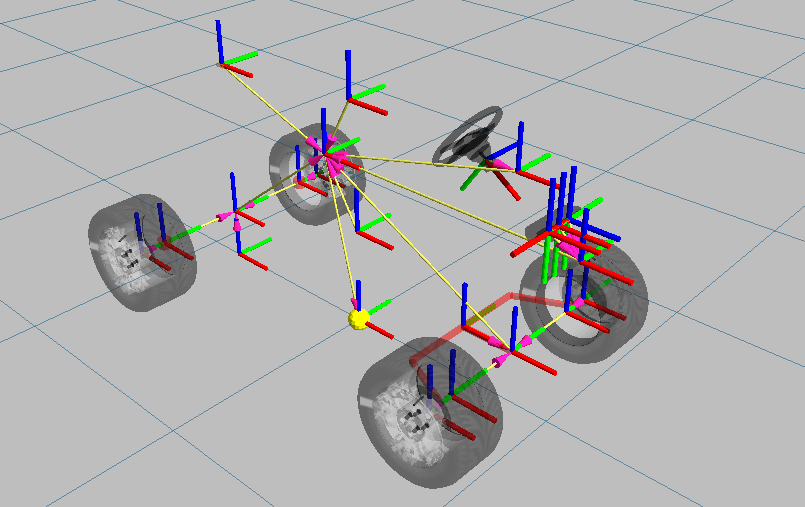
\includegraphics[width=6cm]{modelo_carina/carina_tf_side_wheels_transp.png}
%	 	\caption{Sistemas de coordenadas de referência (TF)}
%	 	\label{fig:tf}
%	\end{minipage}
%	\begin{minipage}[b]{0.5\linewidth}
%	    \centering
%	    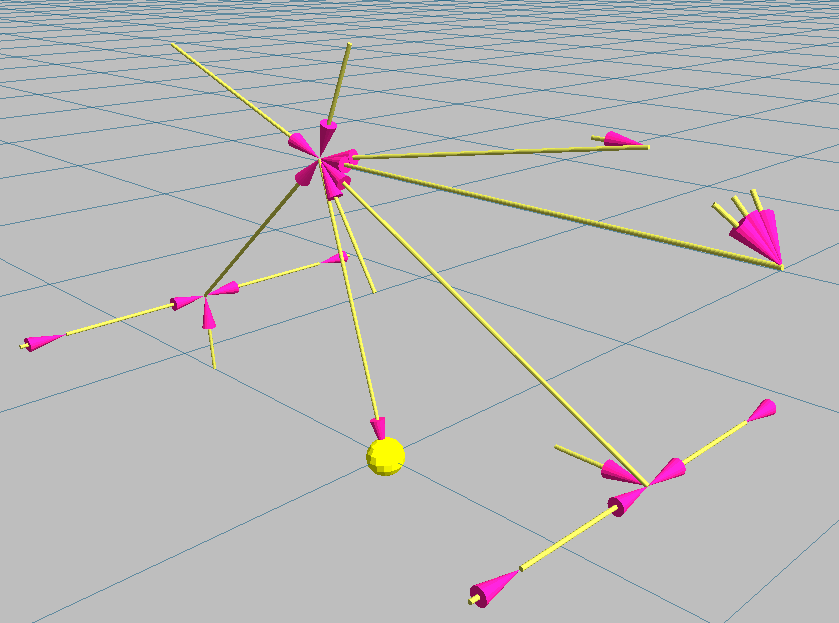
\includegraphics[width=6cm]{modelo_carina/carina_tf_side_no_axis.png}
%	 	\caption{Representação em árvore}
%	 	\label{fig:tree}
%	\end{minipage}	
%\end{figure}

%Most physical simulation libraries uses the concept of links and joints
%to describe physical relations of the structures of a body. A joint describe
%a relation between links and both can present physical properties like friction
%coefficients, elasticity and masses. These links and joint represent physical
%relations and mechanical structures of the robot like arms, wheels and its
%axels and so on. To describe links and joints relations, a graph representation
%would be more suited and this makes the URDF tree structure a little limiting
%to fully describe the model.

%Gazebo has its own XML description language called SDF to model scenarios and
%robots with its physics parameters. SDF share some compatibility with URDF and
%URDF can be extended with Gazebo specific tags, this way the same robot
%description can be shared between ROS and Gazebo. The Gazebo specific modelling
%descriptions are used to plug sensors and controllers to the virtual model and
%also allows describing some mechanical restrictions not permited by the tree
%structure of URDF, like the case in the CaRINA model where the Ackermann
%Geometry was modelled (\fig{fig:ackermann}).

%\begin{figure}[h!]
%	\begin{minipage}[b]{1\linewidth}
%	    \centering
%	    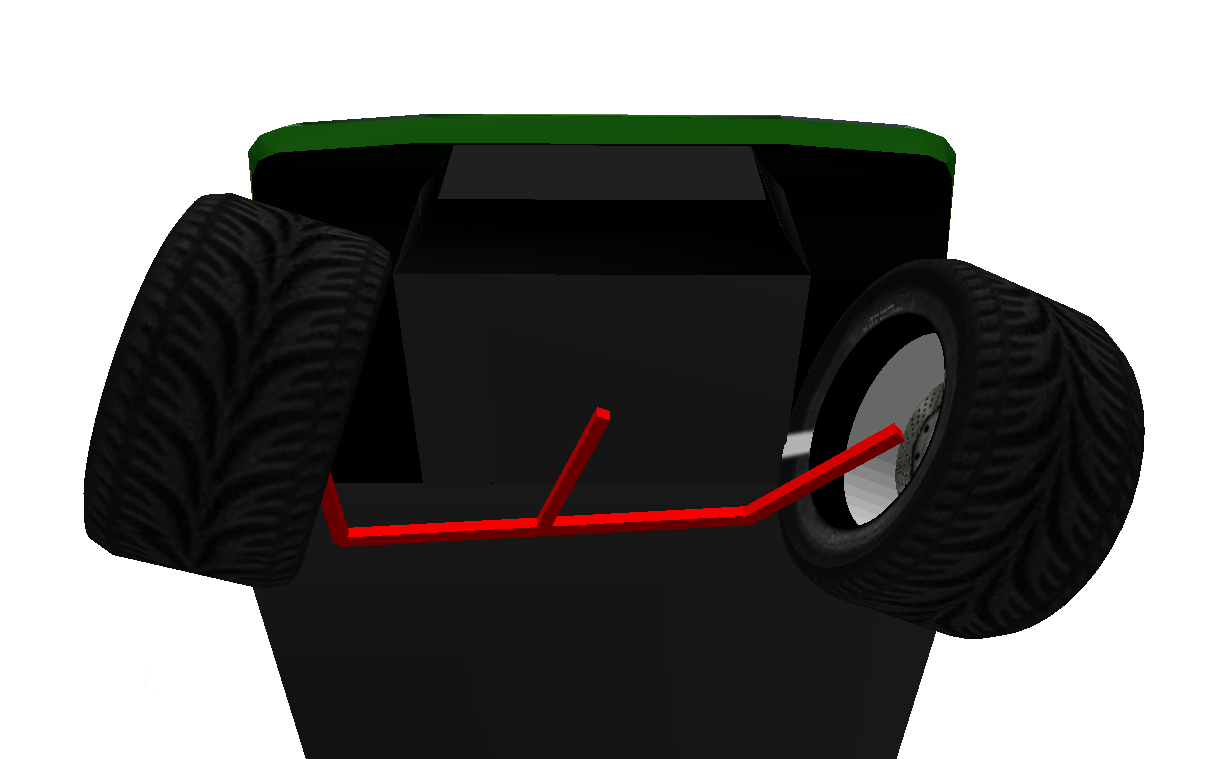
\includegraphics[width=6cm]{modelo_carina/carina_rviz_steering.png}
%	 	\caption{Ackermann steering geometry modelled in simulation}
%	 	\label{fig:ackermann}
%	\end{minipage}
%\end{figure}

%We also put on the virtual model a suspension mechanism independant on each
%wheel. Since our intentions are not to simulate the mechanical behaviour of the
%car itself but our autonomous navigation systems, the suspension is an
%aproximation model just enought to enable us to simulate on uneven terrains
%avoiding the kicking collision effect with the ground caused by the ridgid body
%physics simulation and keeping the four wheels in contact with the ground to
%avoid loss of traction, splipages and unstable poses of the vehicle that
%diverges from real situations. One other effect desired from the simulated
%suspension is the balancing of the vehicle when bending, accelareting and
%breaking, that will have a direct effect on the sensors reading and be more
%close to real situations. This give us a better simulated IMU data with a more
%realistic associated noise (\fig{fig:uneven}).

%\begin{figure}[ht]
%	\begin{minipage}[b]{1\linewidth}
%	    \centering
%	    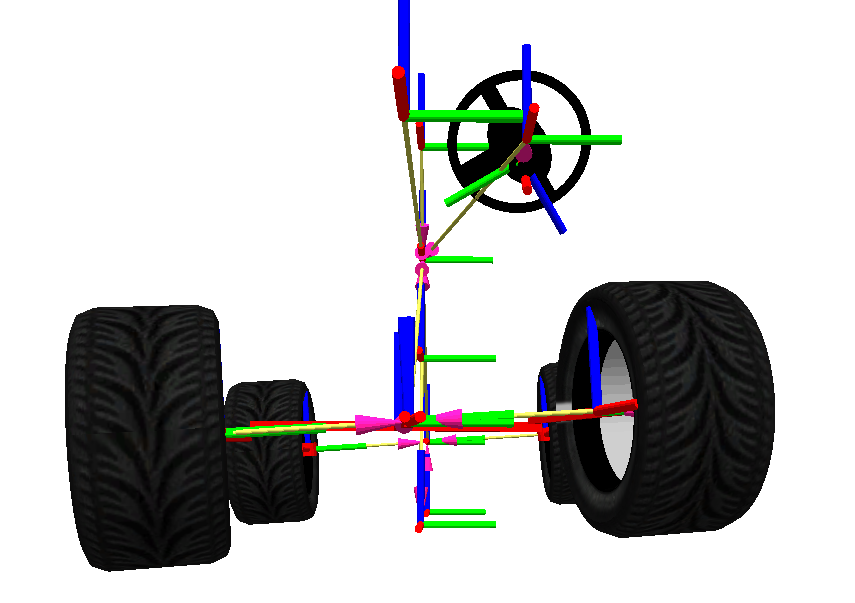
\includegraphics[width=8cm]{modelo_carina/carina_rviz_uneven_susp.png}
%	 	\caption{Suspension effect on an uneven terrain}
%	 	\label{fig:uneven}
%	\end{minipage}
%\end{figure}

\subsection{Arquitetura}

Para o desenvolvimento do sistema e execução no ambiente real também será
utilizada a plataforma ROS, pois ela foi elaborada tendo como um dos propósitos
a padronização de uma interface para dispositivos reais e simulados. Isto
permite o desenvolvimentos dos algoritmos de forma independente da fonte dos
dados.

A arquitetura do sistema de navegação será baseado no modelo geral do ROS
conforme a \fig{fig:arq}.

%OSORIO

%> O ideal é ter figuras em Português, evitando textos em inglês (inclusive na
% tabela abaixo na figira onde apresenta a notação adotada)

%> Seria necessário um texto comentando e detalhando o que representa esta
% figura e seus componentes.

%\vspace{1cm}

%ao mesmo tempo que o custo computacional associado

\begin{figure}[!h]
  	\centering
%	\begin{minipage}[b]{1.0\linewidth}
	    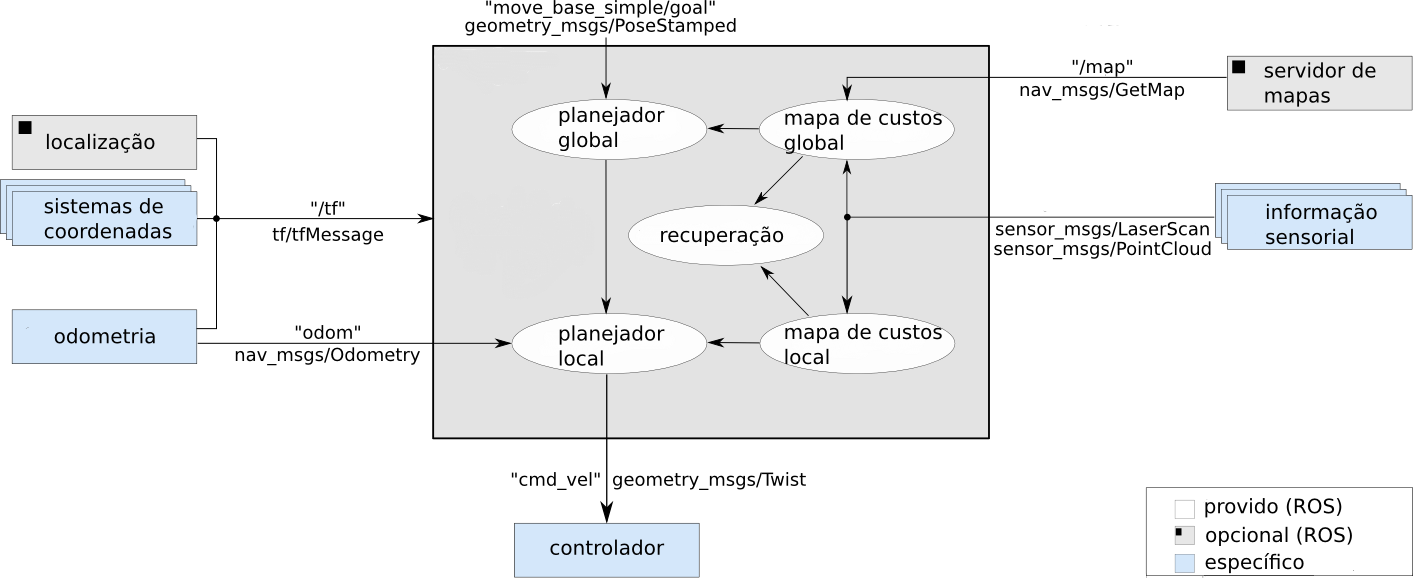
\includegraphics[width=\textwidth,height=8cm]{images/overview_tf_pt.png}
	 	\caption{Arquitetura geral do sistema de navegação.}
		\fonte{adaptado de: www.ros.org}
	 	\label{fig:arq}
% 	\end{minipage}
\end{figure}

Esta arquitetura se baseia em um comportamento deliberativo em relação ao
mapeamento global e um comportamento reativo associado ao mapeamento local. O
serviço de mapa deve fornecer informações de ocupação do espaço, geralmente
discretizado em livre, ocupado e desconhecido. Estes atributos são utilizados no
cálculo dos custos utilizado pelo algoritmo de geração de trajetória. Estes
custos são mantidos pelos mapas de custos e atualizados de acordo com as
informações sensoriais que são constantemente analisadas. 

Nesta arquitetura os componentes específicos dizem respeito ao veículo
e sensores utilizados. Já os componentes providos pela plataforma ROS requerem
as devidas parametrizações e a escolha dos algoritmos adequados para o problema
que ainda estão sendo estudados.

%Os algoritmos de geração de trajetória baseados em amostras tem sido adotado em
%robótica móvel com maior ênfase principalmente pela aplicabilidade prática,
% este tipo de abordagem leva em consideração a cinemática do veículo gerando
%trajetórias realistas com custo computacional baixo \cite{ompl}.

%Por se tratar de uma plataforma aberta todos componentes podem ser customizado
% e adaptados 
%Para a localização já foi 

%A primeira tarefa realizada no projeto foi a modelage do veículo para
%utilização no simulador, esta modelagem contempla a cinemática do veículo no
% modelo Ackerman, onde a angulação das rodas dianteiras são independentes em relação ao
%ângulo de esterçamento do veículo \fig{fig:ackerman}. Esta modelagem também
%contempla os sensores presentes no veículo real que serão utilizados no
% projeto.

%Uma etapa necessária para a navegação é a odometria do veículo, esta odometria
%foi implementada baseando-se nas informações provenientes da contagem de
%rotações da roda juntamente com a medição do angulo de giro da barra de
% direção.




\section{Forma de Análise dos Resultados}

Os resultados serão analisados comparativamente com as soluções já desenvolvidas
no LRM e em comparação com projetos semelhantes e relacionados. Além disto,
serão avaliadas e comparadas as diferentes abordagens adotadas neste estudo,
como por exemplo, comparando a abordagem baseada em VFH com RNAs. Outro quesito
a ser avaliado é o desempenho geral do sistema, onde serão realizadas medições e
avaliações dos tempos de processamento e do desempenho alcançados.

%A adaptabilidade e robustez final do resultado para as áreas de interesse e aplicação citadas nesta
%proposta irá indicar o grau de sucesso atingido. As necessidades de melhorias e a delineação de
%avanços que devem ser alcançados poderão servir de base para novos projetos, constituindo um
%avanço na prospecção tecnológica para o desenvolvimento de um sistema eficiente e robusto de
%navegação autônoma.

A métrica quantitativa mais utilizada para este tipo de sistema são as
frequências em que se permite executar os algoritmos. No caso de imagens a taxa
é dada em FPS (imagens por segundo). Estas taxas tem como principal papel
expressar os resultados de forma que possam ser utilizados para verificar se é
possível construir um sistema tempo real. Uma outra métrica relevante para
categorizar os métodos é uma avaliação qualitativa de quão paralelizável é o
algoritmo utilizado. Esta métrica geralmente acaba sendo apresentada de forma
implícita na descrição da estrutura do algoritmo.

%Para análises estatísticas geralmente são necessários critérios  

%OSORIO
% A validação por simulação permite também gerar situações mais variadas e
% avaliar os limites e capacidades do sistema proposto: variando 
% a densidade/quantidade de obstáculos presentes no ambiente; avaliando a
% quantidade de colisões que podem vir a ocorrer em determinadas situações; 
% verificando em que situações um obstáculo pode vir a não ser detectado; e
% assim por diante.

A primeira etapa consistem em avaliar o sistema em ambiente simulado. A
validação por simulação permite gerar diversas situações desejadas para testar
variados comportamentos sem a necessidade de criá-las no ambiente real, o que
dependendo do cenário pode ser arriscado. A simulação permite maior controle
sobre o ambiente permitindo cenários mais propícios e menos propícios afim de
verificar a robustez do sistema. As análises em ambiente real serão comparadas
com os testes efetuados em simulação permitindo uma avaliação do desempenho,
tanto da qualidade das trajetórias geradas como a capacidade de desvio de
obstáculos.

%OSORIO
%> As "considerações finais" deste capítulo podem ser uma lista da principais
%contribuições esperadas deste trabalhos descritas sobre a forma de uma lista de
% itens.

\section{Contribuições Esperadas}

As principais contribuições acadêmico-científicas esperadas deste trabalho são: 

\begin{enumerate}[i.]

\item adaptação e aperfeiçoamento dos algoritmos para a geração em “tempo real”
de mapas de disparidade, obtendo estes mapas a partir de um par de imagens
capturadas pela câmera estéreo;

\item proposta e desenvolvimento de algoritmos para a obtenção de mapas locais
de navegabilidade com informações espaciais (3D), onde o espaço tridimensional
será dividido em regiões e estas regiões serão identificadas como sendo
navegáveis ou não navegáveis;

\item aperfeiçoamento de técnicas para a navegação baseada no uso de GPS,
bússola e mapas locais de navegabilidade, onde as pesquisas previamente
desenvolvidas para detectar e desviar de obstáculos com o uso de mapas 2D, serão
estendidas a fim de trabalhar com mapa de navegabilidade/ocupação em 3D. Deste
trabalho resultará um sistema com possibilidade de aplicação prática em
importantes tarefas de navegação autônoma, como por exemplo, em sistemas
voltados para aplicações agrícolas e em sistema de combate a incêndio em
florestas, tarefas estas que podem ser perigosas para o ser humano (por exemplo,
exposição prolongada aos produtos químicos de defensivos agrícolas, e
combate/contato direto com fumaça e incêndios).

\end{enumerate}
